\section{Approach for Decomposition and Collaboration}
For a given \emph{IMCL} program $Prog_{ori}$, we can get an AST(Abstract Syntax Tree) which contains details of its statements by an open source grammar parser tool, ANTLR\cite{ANTLRbook}.
Then, we can get the corresponding CFG(Control Flow Graph) and DFG(Data Flow Graph) based on AST.
% CFG is a  Through the lexical analysis and grammar analysis of AST, we can obtain the CFG of the $Prog_{ori}$ and variables of each statement.
% For every variable that appear in CFG, there could be data dependence in it. So making sure the $DD_{post}$ of each statement can help get the SDG of $Prog_{ori}$.\\
%\medskip
%\textbf{AST:} \ The abstract syntax tree(AST) of IMCL program. Based on AST, we can obtain the relationship between the statements of the IMCL program by lexical analysis and grammar analysis.
A $CFG = \langle N, E \rangle$ is a directed graph, where \emph{N} is a set of nodes, and $E \subseteq N \times N$ is the set of edges while \emph{DFG} is a data-flow digraph structure. If $(n_1,n_2) \in E$, then $n_2$ is an immediate successor of $n_1$.

During the construction of CFG, we can get the information of each node. For each node $n$, we can have the following three sets: \emph{REF(n)}, \emph{DEF(n)} and \emph{INFL(n)}. \emph{REF(n)} is the set of variables whose values are used at n, and \emph{DEF(n)} is the set of variables whose values are changed at n. \emph{INFL(n)} is the set of nodes transitively control dependence on $n$, and it will not be empty only when $n$ has more than one immediate successor(for example, $n$ is a branch statement or a loop node).

There is a \emph{post} data-dependency($DD_{post}$) set of nodes for every node in the DFG, which is described as follow:\\
\begin{displaymath}
    \forall x \in DD_{post}(n), \ REF(x) \cap DEF(n) \neq \emptyset
\end{displaymath}
The $DD_{post}$(n) denotes that there are some nodes that are all data-depended on node $n$.
% For example, $DD_{post}(m) = \{2,6\}$, which means that at least one variable in both statement 2 and 6 are depended on statement $m$, respectively.

\textbf{SDG:} \ The \emph{System Dependence Graph}(SDG), a graph representation of system model with data dependence and control dependence, and which is based on \emph{CFG} and \emph{DFG}:
\begin{displaymath}
    SDG :=  \bigcup_{i=1}^{N} (CFG \oplus DD_{post}(i))
\end{displaymath}
which denotes that the SDG is a combination of CFG and all $DD_{post}$(i) that data-depended on every statement.

%In our research, we implement the decomposition and collaboration algorithms in a tool. The Fig.\ref{fig_approach} shows the approach to decompose the complicated system model to some collaborated sub-systems based on the SDG.

%\TODO{TODO}{repalce the picture Fig 1}


There are five basic terms for approach:
\begin{itemize}
  \item \textbf{Original Model:}\  The Original model is an \emph{IMCL} model $Prog_{ori}$ given at the beginning time, which is the description of an industrial control system.
  \item \textbf{Statement:}\ The $statement$ is the minimum computational task level for the program. Therefore, the $Prog_{ori}$ can be treated as a set of statements.
  \item \textbf{Resource Constraints:}\ It describes the constraints that physical resources are limited available for specific CUs.
  \item \textbf{Decomposition Model:}\  It is the multiple models that all of the statements in \emph{Original Model} are decompose to specified $CU$. In other words, it is transformed from a $Prog_{ori}$ with the resource constraint to the set of $Prog_{cu}$ for every \emph{CU}.
  \item \textbf{Collaboration Model:}\  Which is a set of the $Prog_{cu}$ interact with each other with communication and synchronization.
\end{itemize}

\begin{figure*}[!ht]
    \centering
        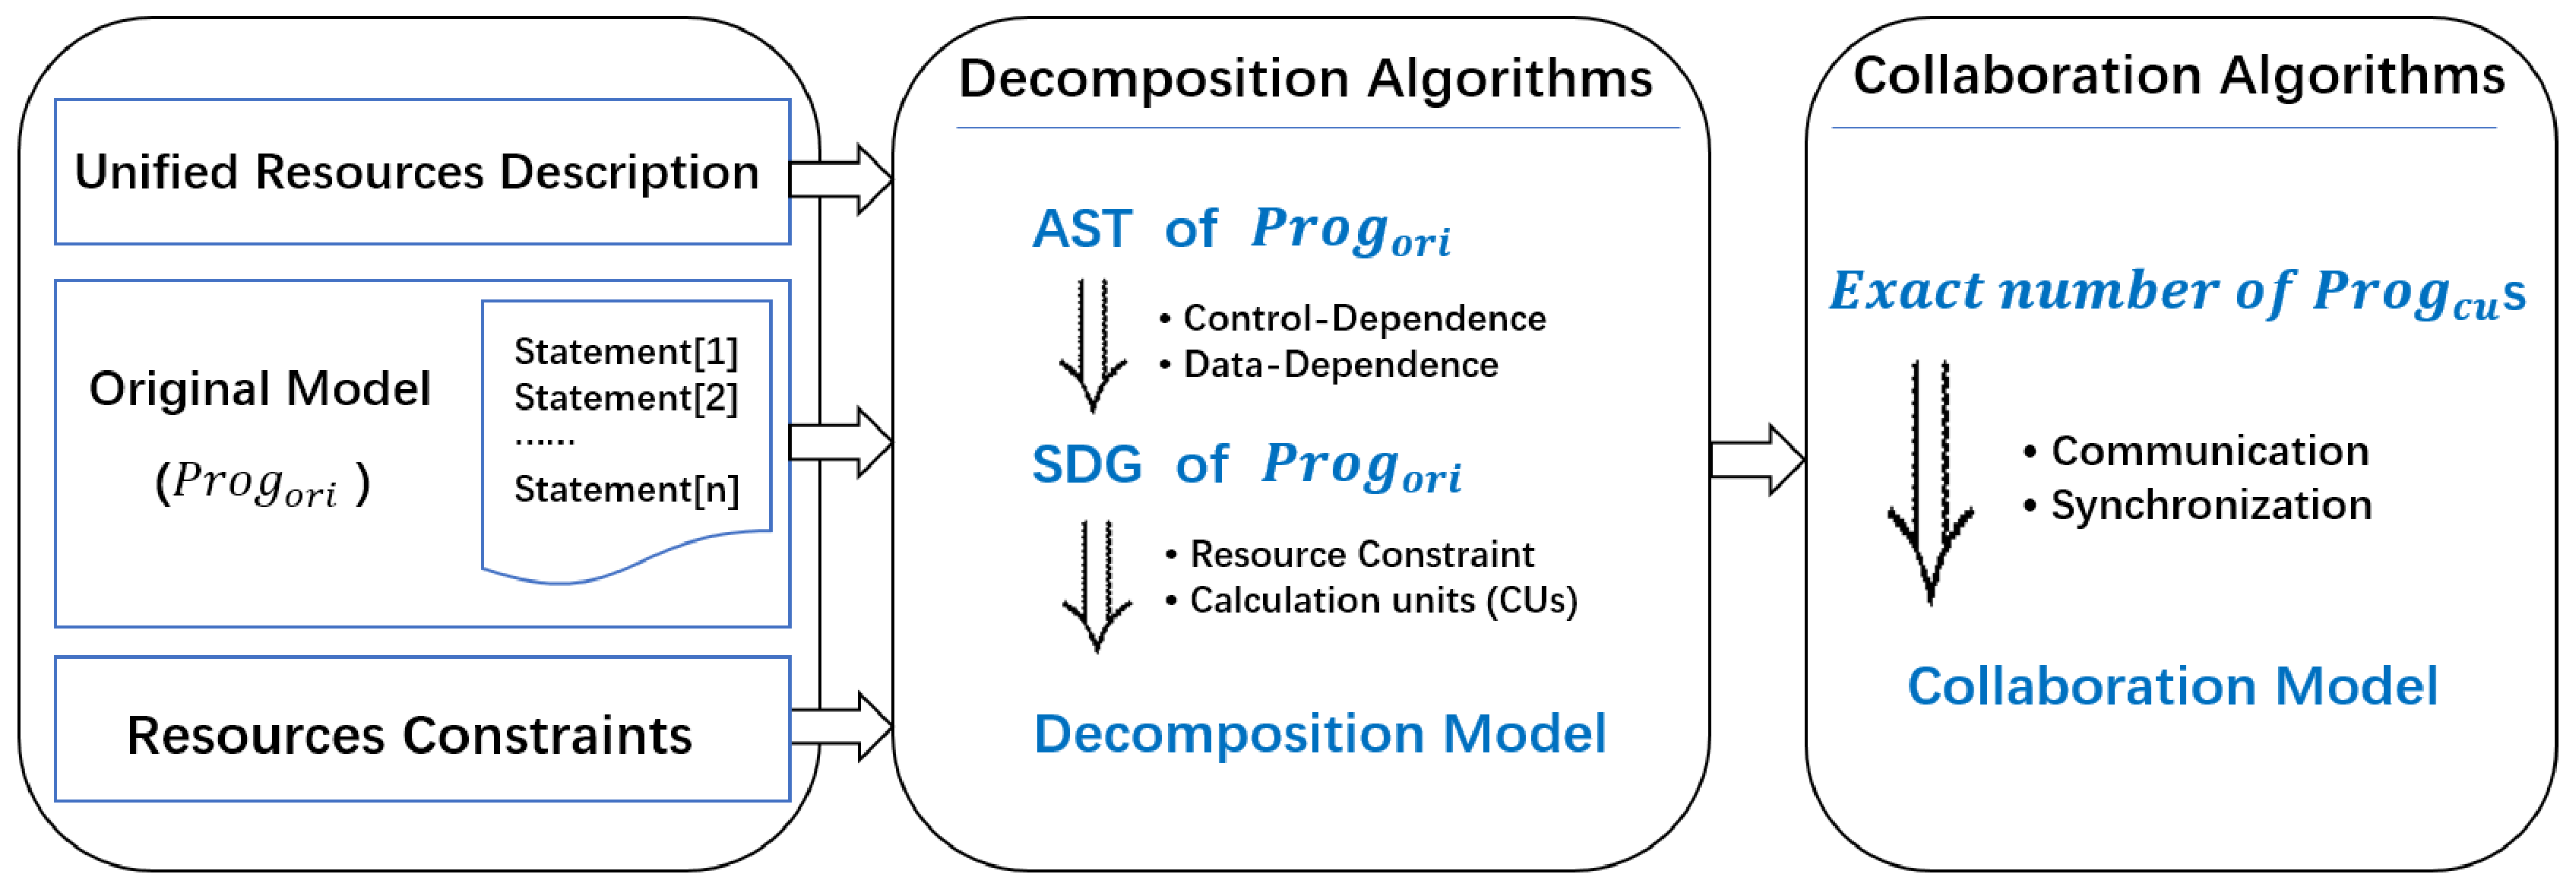
\includegraphics[height=1.6in, width=4.5in]{fig_Approach}
    \caption{Overview of approach for decomposition and collaboration }\label{fig_approach}
\end{figure*}

Fig \ref{fig_approach} is the overview of the approach for decomposition and collaboration that we have implemented in our tool. For one industrial control system, we model the physical resources and system as one \emph{Original Model} ($Prog_{ori}$) . Based on the SDG of $Prog_{ori}$, we implement the decomposition and collaboration algorithms to decompose the \emph{Original Model} to the \emph{Collaboration Model} with the resource constraints.

